\documentclass[10pt]{article}
\usepackage[utf8]{inputenc}
\usepackage[czech]{babel}
\usepackage{a4wide}
\usepackage{graphicx}

\newcommand{\labtitle}[4]{
	\begin{titlepage}
		\begin{center}
			\mbox{} \\[4cm]
			{\huge {#1}} \\[2cm]
			{\Large #2}  % \\[.2cm]
			{\large #3 } \\[.7cm]
			{\normalsize měřeno #4}
		\end{center}
	\end{titlepage}
}


\begin{document}

% -- title page -- %
\labtitle{Studium solárního článku}
 {Tomáš Maršálek}
 {(A10B0632P)}
 {31.\,října 2011}
% -- title page -- %


\section{Měřící potřeby a přístroje}
solární baterie, termoelektrická baterie, univerzální měřící zesilovač, reostat
330~$\Omega$~1~A, žárovka 220~V / 120~W s~reflektorem, digitální multimetr

\section{Naměřené hodnoty}

\begin{scriptsize}
\begin{minipage}[t]{.5\textwidth}
\vspace{0pt}
\begin{tabular}[b]{|c|c|c|c||c|}
\hline
a~[cm] & U~[mV] & U$_0$~[V] & I$_f$~[mA] & E~[Wm$^{-2}$] \\
\hline
50  & 38.8 & 2.10  & 90.0 & 801.6 \\
55  & 35.2 & 2.08  & 80.8 & 727.2 \\
60  & 31.8 & 2.06  & 73.5 & 657.0 \\
65  & 26.1 & 2.05  & 67.0 & 539.2 \\
70  & 23.5 & 2.02  & 56.5 & 485.5 \\
80  & 21.5 & 2.01  & 52.0 & 444.2 \\
85  & 18.7 & 2.00  & 48.0 & 386.3 \\
90  & 18.0 & 1.999 & 44.7 & 371.9 \\
95  & 16.7 & 1.998 & 41.3 & 345.0 \\
100 & 15.2 & 1.979 & 38.6 & 314.0 \\
\hline
\end{tabular}
\end{minipage}
\begin{minipage}[t]{.5\textwidth}
\vspace{0pt}
\begin{tabular}[b]{|c|c|c|c|c|c|}
\hline
\multicolumn{2}{|l|}{E = 801 $Wm^{-2}$} & 
\multicolumn{2}{l|}{E = 539 $Wm^{-2}$} &
\multicolumn{2}{l|}{E = 444 $Wm^{-2}$} \\

\hline
U$_1~[V]$ & I$_1$~[mA] & U$_2$~[V] & I$_2$~[mA] & U$_3$~[V] & I$_3$~[mA] \\
\hline
0.23 & 90.1 & 0.25 & 67.1 & 0.23 & 52.0 \\
0.38 & 90.3 & 0.44 & 67.3 & 0.32 & 52.1 \\
0.66 & 90.0 & 0.67 & 67.2 & 0.65 & 52.0 \\
0.94 & 89.7 & 0.84 & 67.1 & 1.12 & 52.0 \\
1.22 & 89.9 & 1.00 & 67.0 & 1.49 & 51.1 \\
1.53 & 89.2 & 1.35 & 60.8 & 1.72 & 41.5 \\
1.72 & 80.3 & 1.58 & 64.6 & 1.68 & 34.7 \\
1.75 & 76.2 & 1.69 & 58.5 & 1.82 & 26.8 \\
1.80 & 65.2 & 1.75 & 53.0 & 1.87 & 17.4 \\
1.80 & 35.1 & 1.85 & 32.9 & 1.91 & 5.9 \\
1.90 & 35.1 & 1.85 & 32.9 & - & - \\
1.92 & 23.8 & 1.90 & 17.7 & - & - \\
1.93 & 20.2 & 1.91 & 10.7 & - & - \\
1.94 & 14.9 & 1.92 & 7.2 & - & - \\
\hline
\end{tabular}
\end{minipage}
\end{scriptsize}

\section{Výpočty}
\subsection{Intenzity}
Závislost napětí a proudu nakrátko na intenzitě ozáření \\
\includegraphics[width=6cm,angle=270]{graf1.eps}
\includegraphics[width=6cm,angle=270]{graf2.eps} \\[1cm]

\noindent
Maximální hodnota napětí naprázdno je $U_{0max} = 2.10$~[V]. \\
Konstanta $C$ ze vztahu $I_f = CE$ je určena pomocí lineární regrese a vychází
$C = 0.1156$.

\subsection{Voltampérmetrové charakteristiky}
\begin{center}
\includegraphics[width=9cm,angle=270]{graf3.eps} \\[1cm]
\end{center}

\subsection{Účinnost}
Účinnost solární baterie zjistíme jako poměr maximálního výstupního výkonu 
a~dopadajícího výkonu na čtyři články, každý s rozměry 2.5~cm $\times$ 5~cm.

Celková plocha baterie je $S = 0.005~m^2$. Dopadající výkon pro $E =
801~Wm^{-2}$ pak bude $P = ES$, tedy $P = 4.005~W$. Maximální výstupní výkon 
pro stejnou intenzitu je $P = 138.116~mW$.

Účinnost je tedy $\eta = 0.035$, tzn. 3.5~\%.

\section{Závěr} 
\end{document}
